\documentclass[11pt]{book} % or report
\usepackage{amsmath}
\usepackage{amsfonts}
\usepackage{amssymb}
\usepackage{geometry}
\geometry{a4paper, margin=1in}
\usepackage{graphicx}
\usepackage[hidelinks]{hyperref}
\usepackage{amsthm}
\usepackage{tikz}
\usepackage{subcaption}
\usetikzlibrary{positioning}
\usepackage{pgfplots} 
\usepackage[ruled,vlined]{algorithm2e} 
\usepackage{dsfont}
\usepackage{graphicx}
\usepackage{mathdesign}
\usepackage{float}
\usepackage{todonotes} 
\usepackage{empheq}
\usepackage{array}
\usepackage[ruled,vlined]{algorithm2e} 



\setlength{\parindent}{0pt}

% \let\stdsection\section
% \renewcommand\section{\newpage\stdsection}

\newcommand\mycommfont[1]{\footnotesize\ttfamily\textcolor{blue}{#1}}
\newcommand\defeq{\stackrel{\mathclap{\normalfont\mbox{def}}}{=}}
\SetCommentSty{mycommfont}

\DeclareMathOperator*{\argmax}{argmax}
\DeclareMathOperator*{\argmin}{argmin}

\newtheorem{theorem}{Theorem}[section]
\newtheorem{lemma}{Lemma}[section]
\newtheorem{definition}{Definition}[section]
\newtheorem{corollary}{Corollary}[section]
\newtheorem{claim}{claim}[section]
\newtheorem{example}{Example}[section]


\newtheorem*{claim*}{Claim}
\newtheorem*{lemma*}{Lemma}
\newtheorem*{corollary*}{Corollary}
\newtheorem*{remark*}{Remark}
\newtheorem*{example*}{Example}
\newtheorem*{examples*}{Examples}
\newtheorem*{definition*}{Definition}



\setcounter{tocdepth}{3}





\begin{document}

\begin{titlepage}
    \begin{center}
     {\huge\bfseries 
     The Five Miracles of Mirror Descent \\}
     % ----------------------------------------------------------------
     \vspace{1.5cm}
     {\Large\bfseries Hadar Tal}\\[5pt]
     hadar.tal@mail.huji.ac.il\\[14pt]
      % ----------------------------------------------------------------
     \vspace{2cm}
     {This paper is a summary of the educational materials and lectures from 
     \begin{itemize}
        \item \textbf{The Five Miracles of Mirror Descent} by Professor Sebastien Bubeck, Microsoft Research (Claire Boyer's notes)
        \item \textbf{Wikipedia}
        \item \textbf{3Blue1Brown} YouTube channel
     \end{itemize}
     }

     \vfill
    {Winter 2024}
    \end{center}
\end{titlepage}


\frontmatter
\tableofcontents

% * * * * * * * * * * * * * * * * * * * * * * * * 
% * * * * * * * * * * * * * * * * * * * * * * * * 
% * * * * * * * * * * * * * * * * * * * * * * * * 
% * * * * * * * * * * * * * * * * * * * * * * * * 
% * * * * * * * * * * * * * * * * * * * * * * * * 
% * * * * * * * * * * * * * * * * * * * * * * * * 
% * * * * * * * * * * * * * * * * * * * * * * * * 
% * * * * * * * * * * * * * * * * * * * * * * * * 
% * * * * * * * * * * * * * * * * * * * * * * * * 
% * * * * * * * * * * * * * * * * * * * * * * * * 
% * * * * * * * * * * * * * * * * * * * * * * * * 
% * * * * * * * * * * * * * * * * * * * * * * * * 
% * * * * * * * * * * * * * * * * * * * * * * * * 
% * * * * * * * * * * * * * * * * * * * * * * * * 
% * * * * * * * * * * * * * * * * * * * * * * * * 
% * * * * * * * * * * * * * * * * * * * * * * * * 
% * * * * * * * * * * * * * * * * * * * * * * * * 
% * * * * * * * * * * * * * * * * * * * * * * * * 
% * * * * * * * * * * * * * * * * * * * * * * * * 

\mainmatter
\chapter{The First Miracle: Robustness}

Let f be a convex function, and let $x^*$ be a minimizer of f. 

\section{Gradient Descent}
\begin{definition}{Gradient Descent} \\
    \begin{equation}
       x_{t+1} = x_t - \eta \nabla f(x_t) 
    \end{equation}
\end{definition}

It holds that:
\begin{equation}
    f(x^*) \geq f(x_t) + \nabla f(x_t) \cdot (x^* - x_t)
\end{equation}

\begin{equation}
    0 \leq f(x_t) - f(x^*) \leq \nabla f(x_t) \cdot (x_t - x^*) 
\end{equation}

\subsection{Analysis of the Gradient Descent Algorithm}

\begin{align*}
    \|a\|^2  &= \|b\|^2 + \|a - b\|^2   \\ 
    \|b\|^2 &= \|a\|^2 - \|a - b\|^2 = \|a\|^2 - ( \|a\|^2 - 2a \cdot b + \|b\|^2  ) = 2 a \cdot b - \|b\|^2
\end{align*}
Then we have:
\begin{align*}
    \| x^* - x_t \|^2 - \| x^* - x_{t+1} \|^2 &= - 2 \eta (x^* - x_t) \cdot \nabla f(x_t) - \eta^2 \| \nabla f(x_t) \|^2 \\
    &= 2 \eta (x_t - x^*) \cdot \nabla f(x_t) - \eta^2 \| \nabla f(x_t) \|^2 \\
    &\geq  2 ( f(x_t) - f(x^*) ) - \eta^2 L^2
\end{align*}

Where the last inequality follows from the convexity and the Lipschitz continuity of $f$. 

\begin{figure}[H]
    \centering
    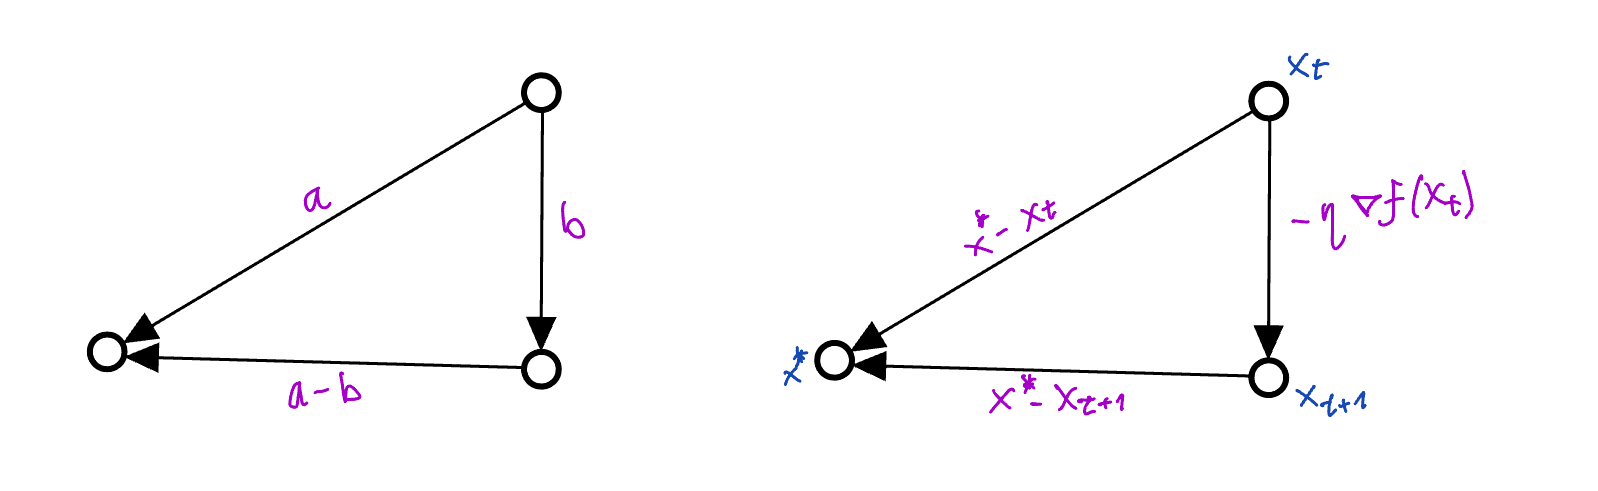
\includegraphics[width=0.8\textwidth]{Figs/vectors_triangle.jpeg}
    \caption{Gradient Descent}
\end{figure}

Then if we sum the above inequality from $t=1$ to $T$, we get:
\begin{align*}
    \sum_{t=1}^T ( f(x_t) - f(x^*) ) &\leq \frac{\|x_1 - x^*\|^2}{2 \eta} + \frac{\eta L^2}{2} T 
\end{align*}

In fact, this is a specific case of the Fundamental Inequality of Optimization. 

\begin{theorem}{Fundamental Inequality of Optimization (unconstrained version)} \\
    Suppose \( x_{t+1} = x_t - \eta g_t \) for all \( t \), where \( g_1, \ldots, g_T \in \mathbb{R}^d \) are arbitrary vectors. Then for all \( x^* \in \mathbb{R}^d \) it holds that
    \[
    \sum_{t=1}^T g_t \cdot (x_t - x^*) \leq \frac{\|x_1 - x^*\|^2}{2\eta} + \frac{\eta}{2} \sum_{t=1}^T \|g_t\|^2.
    \]
\end{theorem}
    
\begin{proof}{Fundamental Inequality of Optimization} \\
    The proof tracks \( \|x_t - x^*\|^2 \) as a ``potential''. First write
    \[
    \|x_{t+1} - x^*\|^2 = \|(x_t - x^*) - \eta g_t\|^2 = \|x_t - x^*\|^2 - 2\eta g_t \cdot (x_t - x^*) + \eta^2 \|g_t\|^2,
    \]
    that is,
    \[
    \|x_t - x^*\|^2 - \|x_{t+1} - x^*\|^2 = 2\eta g_t \cdot (x_t - x^*) - \eta^2 \|g_t\|^2.
    \]
    Summing over \( t = 1, \ldots, T \) and telescoping terms, we obtain
    \[
    \|x_1 - x^*\|^2 - \|x_{T+1} - x^*\|^2 = 2\eta \sum_{t=1}^T g_t \cdot (x_t - x^*) - \eta^2 \sum_{t=1}^T \|g_t\|^2.
    \]
    Organizing terms, we conclude:
    \[
    \sum_{t=1}^T g_t \cdot (x_t - x^*) \leq \frac{\|x_1 - x^*\|^2 - \|x_{T+1} - x^*\|^2}{2\eta} + \frac{\eta}{2} \sum_{t=1}^T \|g_t\|^2. \quad 
    \]
\end{proof}

\bigbreak


\todo[inline]{SGD , choosing eta} 
    

% * * * * * * * * * * * * * * * * * * * * * * * * 
% * * * * * * * * * * * * * * * * * * * * * * * * 
% * * * * * * * * * * * * * * * * * * * * * * * * 
% * * * * * * * * * * * * * * * * * * * * * * * * 
% * * * * * * * * * * * * * * * * * * * * * * * * 
% * * * * * * * * * * * * * * * * * * * * * * * * 
% * * * * * * * * * * * * * * * * * * * * * * * * 
% * * * * * * * * * * * * * * * * * * * * * * * * 
% * * * * * * * * * * * * * * * * * * * * * * * * 
% * * * * * * * * * * * * * * * * * * * * * * * * 
% * * * * * * * * * * * * * * * * * * * * * * * * 
% * * * * * * * * * * * * * * * * * * * * * * * * 
% * * * * * * * * * * * * * * * * * * * * * * * * 
% * * * * * * * * * * * * * * * * * * * * * * * * 
% * * * * * * * * * * * * * * * * * * * * * * * * 
% * * * * * * * * * * * * * * * * * * * * * * * * 
% * * * * * * * * * * * * * * * * * * * * * * * * 
% * * * * * * * * * * * * * * * * * * * * * * * * 
% * * * * * * * * * * * * * * * * * * * * * * * * 

\chapter{The Second Miracle: Potential Based}

\section{Experts Problem}

At each time step, the player picks an action $I_t \in [n]$ (we have n experts) and the adversary picks a loss vector $l_t \in {0,1}^n$. 
The player incurs loss $l_t(I_t)$ and the goal is to minimize the regret:
\begin{equation}
    \text{Regret}_T(i) = \sum_{t=1}^T \left( l_t(I_t) - l_t(i) \right)
\end{equation}

We consider the case where in each time step the player chooses an action from a distribution $\vec{p}$ over the $n$ experts (a vector from the simplex):
\begin{equation*}
    \vec{p} \in \mathcal{K} := \bigtriangleup_n = \{ \vec{p} \in \mathbb{R}_+^n : p_i \geq 0, \sum_{i=1}^n p_i = 1 \}
\end{equation*}

\subsubsection{Approach 1: Gradient Descent}
We can use gradient descent on $f_t(\vec{p}_t) = \vec{l_t} \cdot \vec{p}$, where $\vec{l_t}$ is the loss vector at time $t$.
It holds that $\nabla f_t(\vec{p}_t) = \vec{l_t}$. We can use the analysis of the gradient descent algorithm for gradient descent of convex functions varying in time.

Let $q \in \bigtriangleup_n$ be any distribution. Then we have:
\begin{align*}
    f_t(q) &\geq f_t(\vec{p}_t) + \nabla f_t(q) \cdot (q - \vec{p}_t) \Longrightarrow \\
    f_t(\vec{p}_t) - f_t(q) &\leq \nabla f_t(q) \cdot (\vec{p}_t - q) 
\end{align*}
Then:
\begin{align*}
    \| q - p_t \|^2 - \| q - p_{t+1} \|^2 &= - 2 \eta (q - p_t) \cdot \nabla f_t(p_t) - \eta^2 \| \nabla f_t(p_t) \|^2  \Longrightarrow \\
    f_t(\vec{p}_t) - f_t(q) &\leq \nabla f_t(q) \cdot (\vec{p}_t - q)  = \frac{1}{2\eta} \left( \| q - \vec{p}_t \|^2  - \| q - \vec{p}_{t+1} \|^2 \right) + \frac{\eta}{2} \| \nabla f_t(\vec{p}_t) \|^2 \Longrightarrow \\ 
    \sum_{t=1}^T \left( f_t(\vec{p}_t) - f_t(q) \right) &\leq \frac{1}{2\eta} \left( \| q - \vec{p}_1 \|^2 - \| q - \vec{p}_{T+1} \|^2 \right)+ \frac{\eta}{2} \sum_{t=1}^T \| \nabla f_t(\vec{p}_t) \|^2 \\
    &\leq \frac{1}{2\eta} \| q - \vec{p}_1 \|^2 + \frac{\eta}{2} \sum_{t=1}^T \| \nabla f_t(\vec{p}_t) \|^2 \\
    &\leq \frac{1}{\eta} + \frac{\eta}{2} T n  = \textbf{O} ( \sqrt{Tn} )
\end{align*}

We have used the facts that: 
\begin{itemize}
    \item Both $q$ and $\vec{p}_1$ are distributions, so $\| q - \vec{p}_1 \|^2 \leq 2$.
    \item $\| \nabla f_t(\vec{p}_t) \|^2 \leq n$ (as the loss vector is in ${0,1}^n$).
\end{itemize}

we can see that in this case, the rate of convergence DO depend on the dimension of the problem, in contrast to the non-varying case.
The fact that the rate of convergence DO NOT depend on the dimension of the problem in GD is one of the reasons why GD is so useful in practice.


\subsubsection{Approach 2: Multiplicative Weights Update (MWU)}

The optimal convergence rate for the experts problem is $\sqrt{T \log n}$, which is achieved by the MWU algorithm.
It is achieved by considering the sparsity of the OPT strategy (which is just a point mass on the best expert). 
We will modify GD such that it will move faster when far from a sparse point.

\medbreak

\todo[inline] {Approach 2: M}


\section{Mirror Descent}

Endow $\mathcal{K}$ with a Riemannian structure: \\
$<\cdot, \cdot>_x$ for each $x \in \mathcal{K}$, the tangent space will be $\mathbb{R}^n$. \\
\begin{align*}
    \text{Before:}\\
    x_{t+1} = x_t - \eta \nabla f(x_t) \rightarrow f(x + dx) &\approx f(x) + \langle \nabla f(x) , dx \rangle \\
    \text{Now:}\\
   f(x + dx) &\approx f(x) + \langle grad_M f(x) , dx \rangle_x
\end{align*}

We will consider $M$ such that $\langle \cdot, \cdot \rangle_x = \nabla^2 \phi [\cdot, \cdot]$, where $\phi$ is a fixed convex function. 
The function $\phi$ encodes the geometry of the space, and this is where the prior information is encoded. We get that:
\begin{align*}
    (dx)^T  \nabla f(x) = \langle grad_M f(x) , dx \rangle_x &= dx^T \nabla^2 \phi(x) grad_M f(x) \Rightarrow \\
    grad_M f(x) &= [\nabla^2 \phi(x)]^{-1} \nabla f(x)
\end{align*}

Idea: $x_{t+1} = x_t - \eta [\nabla^2 \phi(x_t)]^{-1} \nabla g_t $ \\
Question: what is the potential? (how do we analyze this algorithm?) \\
Miracle: the potential is the Bregman divergence of $\phi$ ($D_{\phi}(x, y) = \phi(x) - \phi(y) - \langle \nabla \phi(y), x-y \rangle_x$) [Nemiroski, 1979] 

\bigbreak

\begin{algorithm}[H]
    \SetNoFillComment
    \SetAlgoLined
    % \KwIn{} 
    % \KwOut{}
    $g : \mathbb{R}_+ \to \mathbb{R}^n$ is a smooth vector field \\
    \begin{align*}
        \frac{d}{dt} x_t &= -[\nabla^2 \phi(x_t)]^{-1} (\eta g(t) + \lambda (t))
    \end{align*}
    Where $\lambda(t) \in N_{\mathcal{K}}(x_t), x(t) \in \mathcal{K}$ is a lagrange multiplier - it is an element of the normal cone of $\mathcal{K}$ at $x_t$. \\
    \caption{Continues time Mirror Descent} \label{Continues time Mirror Descent}

    This is the same as the following: 
    \begin{align*}
        x(t + dt) = \argmin_{x \in \mathcal{K}} \left\{ \eta g(t) \cdot x + \frac{1}{2} \| x - x(t) \|^2_{x(t)} \right\}
    \end{align*}
    where $\| h \|^2_x = \nabla^2 \phi(x) [h, h]$ is the norm induced by the Riemannian metric. \\
\end{algorithm}

It is the same as the proximal view of GD, except that the proximal operator is with respect to the Riemannian metric.
Recall that in the proximal view of GD, we have:

\begin{algorithm}[H]
    \caption{Proximal Point method} \label{alg:proximal_point_method}
    Given a function \( f \colon \mathbb{R}^d \to \mathbb{R} \) and step size \( \eta > 0 \), compute:
    \[ x_{t+1} = \text{prox}_{h_t,\eta}(x_t), \quad t = 1, 2, \ldots \]
    where \( h_t \colon \mathbb{R}^d \to \mathbb{R} \) are convex functions such that
    \[ \forall x \in \mathbb{R}^d \colon h_t(x) \leq f(x) \leq h_t(x) + \frac{\beta}{2} \| x - x_t \|^2. \]    
\end{algorithm}
That is: \[ x_{t+1} = \argmin_{x \in \mathbb{R}^d} \left\{ f(x_t) + \nabla f(x_t) \cdot (x - x_t) + \frac{1}{2\eta} \| x - x_t \|^2 \right\} \] 
and in MD instead of $\eta$ as a denominator of the distance, we control the ratio by a coefficient $\eta$ of the gradient.

\bigbreak

\begin{theorem}{\textbf{$x(t)$ exists and is unique}} \\
    The solution to the Mirror Descent algorithm exists and is unique.
\end{theorem}

\begin{proof}{\textbf{$x(t)$ exists and is unique}} \\
    \begin{align*}
        D_{\phi}(y, x(t)) &= \phi(y) - \phi(x(t)) - \nabla \phi(x(t)) \cdot (y - x(t)) \\
        \frac{d}{dt}D_{\phi}(y, x(t)) &=  - \nabla \phi(x(t)) \cdot \frac{d}{dt} x(t)  - \nabla^2 \phi(x(t)) \frac{d}{dt} x(t) \cdot (y - x(t)) - \nabla \phi(x(t)) \cdot (- \frac{d}{dt} x(t)) \\
        &= - \nabla^2 \phi(x(t)) \cdot \frac{d}{dt} x(t) \cdot (y - x(t)) \quad (- [\nabla^2 \phi(x(t))] \cdot \frac{d}{dt} x(t) = (\eta g(t) + \lambda(t))) \\
        &= (\eta g(t) + \lambda(t)) \cdot (y - x(t)) \quad (y \in \mathcal{K} \text{ and } \lambda(t) \in N_{\mathcal{K}}(x(t)) \Rightarrow \lambda(t) \cdot (y - x(t)) \leq 0) \\
        &\leq \eta g(t) \cdot (y - x(t)) 
    \end{align*}
\end{proof}

We can think that $g(t) \cdot y $ is what OPT would have pay at time $t$, and $g(t) \cdot x(t)$ is what we pay.
If we pay more than OPT, then the Bregman divergence will decrease and we will move towards OPT.
We get that for any $y \in \mathcal{K}$:
\begin{align*}
    \int_0^T g(t) \cdot (x(t) - y) dt &\leq \frac{D_{\phi} (y, x(0))}{\eta}
\end{align*}

\begin{itemize}
    \item Previously we had 2 terms in the RHS - one for the range and one for the variance, 
    now we have only one term for the range, because we are in a continuous time setting).
    \item By itself, this theorem is meaningless, we can always speed up the time by making $\phi$ smaller (and the Bregman divergence smaller).
\end{itemize}

Discrete time version: \\
\begin{align*}
    \text{discretize } \frac{d}{dt} x(t) &= -[\nabla^2 \phi(x(t))]^{-1} \cdot g(t) \iff \nabla^2 \phi(x(t)) \frac{d}{dt} x(t) = -g(t) \\
    \iff \frac{d}{dt} \nabla \phi(x(t)) &= -g(t)
\end{align*}

Then we get that:
\begin{align*}
    \nabla \phi(x(t+1)) = \nabla \phi(x(t)) - \eta g(t)
\end{align*}

In GD, we have that $x_{t+1} = x_t - \eta \nabla f(x_t)$, and in MD we have that $\nabla \phi(x_{t+1}) = \nabla \phi(x_t) - \eta g(t)$.
We can think of it as - instead of doing an update in the primal space, we do an update in the dual space. \\
Moreover, GD didn't really make sense since $x_t$ was a primal point and $\nabla f(x_t)$ was a dual point (it was a linear functional) - 
so we added primal and dual points, which was ok just in finite dimensions. \\
Mirror Descent fixes this issue - it first map the primal point to the dual space, then do the update in the dual space, and then map back to the primal space.


% * * * * * * * * * * * * * * * * * * * * * * * * 
% * * * * * * * * * * * * * * * * * * * * * * * * 
% * * * * * * * * * * * * * * * * * * * * * * * * 
% * * * * * * * * * * * * * * * * * * * * * * * * 
% * * * * * * * * * * * * * * * * * * * * * * * * 
% * * * * * * * * * * * * * * * * * * * * * * * * 
% * * * * * * * * * * * * * * * * * * * * * * * * 
% * * * * * * * * * * * * * * * * * * * * * * * * 
% * * * * * * * * * * * * * * * * * * * * * * * * 
% * * * * * * * * * * * * * * * * * * * * * * * * 
% * * * * * * * * * * * * * * * * * * * * * * * * 
% * * * * * * * * * * * * * * * * * * * * * * * * 
% * * * * * * * * * * * * * * * * * * * * * * * * 
% * * * * * * * * * * * * * * * * * * * * * * * * 
% * * * * * * * * * * * * * * * * * * * * * * * * 
% * * * * * * * * * * * * * * * * * * * * * * * * 
% * * * * * * * * * * * * * * * * * * * * * * * * 
% * * * * * * * * * * * * * * * * * * * * * * * * 
% * * * * * * * * * * * * * * * * * * * * * * * * 

\chapter{The Third Miracle: }

\section{Coupon Collector Phenomenon}

The coupon collector's problem is a classic example of a problem in probability theory that has applications in various fields such as computer science, 
combinatorics, and stochastic processes. 
The problem describes a scenario where a collector wishes to gather one of each type of coupon, 
and each coupon type is equally likely to be obtained at each trial.

\begin{definition}{\textbf{Coupon Collector Problem}} \\
The \emph{Coupon Collector Problem} considers a scenario with \( n \) different types of coupons.  \\
Each time a coupon is collected, it is of a type chosen uniformly at random from the \( n \) types. \\
The problem is to determine the expected number of coupons that must be collected before having at least one of each type.
\end{definition}

\begin{theorem}{\textbf{Expected Number of Trials for Coupon Collection}} \\
Let \( T \) be the random variable representing the number of trials needed to collect all \( n \) types of coupons. \\ 
Then the expected value of \( T \) is \( E[T] = n \cdot H_n \), where \( H_n \) is the \( n \)-th harmonic number defined as \( H_n = \sum_{k=1}^{n} \frac{1}{k} \).
\end{theorem}

\begin{proof}
The collection process can be broken into \( n \) stages, where stage \( i \) represents the collection of the \( i \)-th new coupon after already
having \( i-1 \) different types. The expected number of trials to collect a new coupon during stage \( i \) is \( \frac{n}{n - (i - 1)} \), 
since there are \( n - (i - 1) \) types not yet collected (geometric distribution). \\ 
Therefore, the expected total number of trials to collect all \( n \) coupons is:

\[
E[T] = \sum_{i=1}^{n} \frac{n}{n - (i - 1)} = n \cdot \sum_{i=1}^{n} \frac{1}{i} = n \cdot H_n.
\]

Hence, the expected number of trials needed to collect all \( n \) types of coupons is \( n \) times the \( n \)-th harmonic number (and is O(n log n)).
\end{proof}


\section{Metrical Task Systems (MTS)}

\begin{definition}{\textbf{MTS (Metrical Task System)} [Borodin, Linial, Saks, '92]} \\
    Let $X$ be a finite metric space. \\
    The player maintains a state $\rho _t \in X$. 
    At time $t+1$ the player receives a task $c_{t+1} : X \to \mathbb{R}_+$ (a cost function) and move to a new state $\rho_{t+1} \in X$. \\
    The movement cost = $dist(\rho_t, \rho_{t+1})$. \\
    The service cost = $c_{t+1}(\rho_{t+1})$.
\end{definition}

Some applications:
\begin{itemize}
    \item \textbf{Self adjusting data structures} - the state is the data structure, the task is the query, the cost is the time to answer the query. \\
    For example: $X = S^n$ set of permutations of $n$ elements, \\
    cost function: $c_{t+1}(\sigma) = \sum_{i=1}^{n'} \mathds{1} (\sigma(i) \neq j)$ and $\sigma(n') = j$ 

    \item \textbf{Power management} - the states are On $/$ Off $/$ Sleep. \\
            $dist(\text{On}, \text{Off}) > dist(\text{On}, \text{Sleep})$. \\
            $c_1(\text{On}) = 0, c_1(\text{Sleep}) = c_1(\text{Off}) = \infty$. \\
            $c_2(\text{On}) = 1, c_2(\text{Sleep}) = \epsilon, c_2(\text{Off}) = 0$. 

    \item Strictly more general than \textbf{prediction with expert advice} - \\
        Imagine that the metric space is trivial (i.e. $dist(x, y) = 0$ for all $x, y$ such that $x \neq y$). \\
        If I don't move, than being evaluated at the next cost function or the current function is the same. 
        The cost that I get when I'm evaluated at the next cost function is upper bounded by the cost that I'm evaluated at the current cost function 
        $+$ the distance that I moved.
\end{itemize}


The type of guarantees:
\begin{itemize}
    \item \textbf{Competitive ratio $\equiv \frac{ALG}{OPT}$} - the ratio between the cost of the algorithm and the cost of the best fixed states in hindsight. 
    \item \textbf{Conjecture in online algorithms} - for any metric space $|X| = n, \quad \exists \quad \mathcal{A} \text{ in } O(\log n)$-competitive algorithm.
        Where the $\log n$ comes from? We have seen that in the experts problem, the optimal rate is $\sqrt{T \log n}$ (also exists in matrix concentration results).
\end{itemize}

Today's Theorem [Bubeck, Cohen, J.Lee, YT.Lee, '18] - $O(\log^2 n)$-competitive algorithm for MTS.
Remember that in some example it is $O(\log n)$ where $n$ is really the parameter of interest, 
but in other examples n is exponential is the parameter of interest (and then we get $O(\log^2 n)$).
$\forall X$ metric space, $\Omega(\frac{\log n}{\log \log n})$ is necessary.

\subsection{Deterministic Strategies on uniform metric}

By "uniform metric" we mean that the distance between any two points is 1. \\
For any deterministic algorithm, it is at least in order of n since the adversary can choose the highest cost function for the algorithm.

Algorithm in $O(n)$-competitive: \\
Stay in state until it accumulates a cost of 1. 
Then mark the state and move to an unmarked state. 
Once everything is marked, I paid $\leq$ 2n and OPT pays at least 1 (since every state is evaluated at least once). So I'm 2n-competitive.

Why is it $\Omega(n)$-competitive? \\
$c_{t+1}(\rho) = +\infty \mathds{1}_{\rho = \rho_t}$.
Over n time steps, the algorithm pays $n$ and OPT pays less than $1$, so the competitive ratio is at least $n$.


\subsection{Randomized Strategies for Uniform Metric}
Randomized algorithms, essential in adversarial models, create uncertainty to prevent adversaries from precisely exploiting the algorithm's state. 
The adversary, lacking knowledge of the algorithm's random location, is forced to target randomly, making the cost sequence unpredictable.

Such randomness leads to bounded accumulated costs over \( n \) iterations. 
The strategy in a uniform metric space dictates that an algorithm stays in a state until accruing a specified cost, 
then moves to a random unmarked state. The expected movement function \( f(n) \), where \( n \) states are unmarked, is given by:
\begin{align*}
f(n) &= \text{the expected number of moves when \( n \) states are unmarked}, \\
&= \frac{1}{n} + f(n-1), \\
&= 1 + \frac{1}{2} + \ldots + \frac{1}{n}, \\
&= \log n + O(1), \\
&= O(\log n).
\end{align*}

Imagine we have n states left to mark, what's the probability that our current state will be the first one to accumulate a cost of 1? $\frac{1}{n}$.
If we are not the first, then we have $n-1$ states left to mark, and the probability that we will be the first to accumulate a cost of 1 is $\frac{1}{n-1}$.
Thus, the expected movements decrease logarithmically with the number of unmarked states. 

What about the lower bound? \\
$c_{t+1}(\rho) = +\infty$ at a random location.
ALG cost over n time is 1 in expectation. 


% * * * * * * * * * * * * * * * * * * * * * * * * 
% * * * * * * * * * * * * * * * * * * * * * * * * 
% * * * * * * * * * * * * * * * * * * * * * * * * 
% * * * * * * * * * * * * * * * * * * * * * * * * 
% * * * * * * * * * * * * * * * * * * * * * * * * 
% * * * * * * * * * * * * * * * * * * * * * * * * 
% * * * * * * * * * * * * * * * * * * * * * * * * 
% * * * * * * * * * * * * * * * * * * * * * * * * 
% * * * * * * * * * * * * * * * * * * * * * * * * 
% * * * * * * * * * * * * * * * * * * * * * * * * 
% * * * * * * * * * * * * * * * * * * * * * * * * 
% * * * * * * * * * * * * * * * * * * * * * * * * 
% * * * * * * * * * * * * * * * * * * * * * * * * 
% * * * * * * * * * * * * * * * * * * * * * * * * 
% * * * * * * * * * * * * * * * * * * * * * * * * 
% * * * * * * * * * * * * * * * * * * * * * * * * 
% * * * * * * * * * * * * * * * * * * * * * * * * 
% * * * * * * * * * * * * * * * * * * * * * * * * 
% * * * * * * * * * * * * * * * * * * * * * * * * 

\chapter{The Fourth Miracle: }

% * * * * * * * * * * * * * * * * * * * * * * * * 
% * * * * * * * * * * * * * * * * * * * * * * * * 
% * * * * * * * * * * * * * * * * * * * * * * * * 
% * * * * * * * * * * * * * * * * * * * * * * * * 
% * * * * * * * * * * * * * * * * * * * * * * * * 
% * * * * * * * * * * * * * * * * * * * * * * * * 
% * * * * * * * * * * * * * * * * * * * * * * * * 
% * * * * * * * * * * * * * * * * * * * * * * * * 
% * * * * * * * * * * * * * * * * * * * * * * * * 
% * * * * * * * * * * * * * * * * * * * * * * * * 
% * * * * * * * * * * * * * * * * * * * * * * * * 
% * * * * * * * * * * * * * * * * * * * * * * * * 
% * * * * * * * * * * * * * * * * * * * * * * * * 
% * * * * * * * * * * * * * * * * * * * * * * * * 
% * * * * * * * * * * * * * * * * * * * * * * * * 
% * * * * * * * * * * * * * * * * * * * * * * * * 
% * * * * * * * * * * * * * * * * * * * * * * * * 
% * * * * * * * * * * * * * * * * * * * * * * * * 
% * * * * * * * * * * * * * * * * * * * * * * * * 

\chapter{The Fifth Miracle: }

% * * * * * * * * * * * * * * * * * * * * * * * * 
% * * * * * * * * * * * * * * * * * * * * * * * * 
% * * * * * * * * * * * * * * * * * * * * * * * * 
% * * * * * * * * * * * * * * * * * * * * * * * * 
% * * * * * * * * * * * * * * * * * * * * * * * * 
% * * * * * * * * * * * * * * * * * * * * * * * * 
% * * * * * * * * * * * * * * * * * * * * * * * * 
% * * * * * * * * * * * * * * * * * * * * * * * * 
% * * * * * * * * * * * * * * * * * * * * * * * * 
% * * * * * * * * * * * * * * * * * * * * * * * * 
% * * * * * * * * * * * * * * * * * * * * * * * * 
% * * * * * * * * * * * * * * * * * * * * * * * * 
% * * * * * * * * * * * * * * * * * * * * * * * * 
% * * * * * * * * * * * * * * * * * * * * * * * * 
% * * * * * * * * * * * * * * * * * * * * * * * * 
% * * * * * * * * * * * * * * * * * * * * * * * * 
% * * * * * * * * * * * * * * * * * * * * * * * * 
% * * * * * * * * * * * * * * * * * * * * * * * * 
% * * * * * * * * * * * * * * * * * * * * * * * * 

\end{document}